% !TEX root = /home/weznon/programming/0207Programming/ftc-programming-guide/main.tex

\documentclass[../main.tex]{subfiles}

\begin{document}
\newpage
%Begin the stuff!
%This version of the template has some placeholder stuff so you can see what it looks like
\section{Control System}
In this section, we will give an overview of the hardware behind the programming aspect of FTC. Note that the information here is specific to using REV stuff; Modern Robotics is something that while (maybe) still legal, you should avoid using.

Rough explanations of the various sensors, motors, etc will be provided. However, detailed information on usage and the like are in a separate section.
\subsection{REV Expansion Hub}
\begin{figure}[H]
    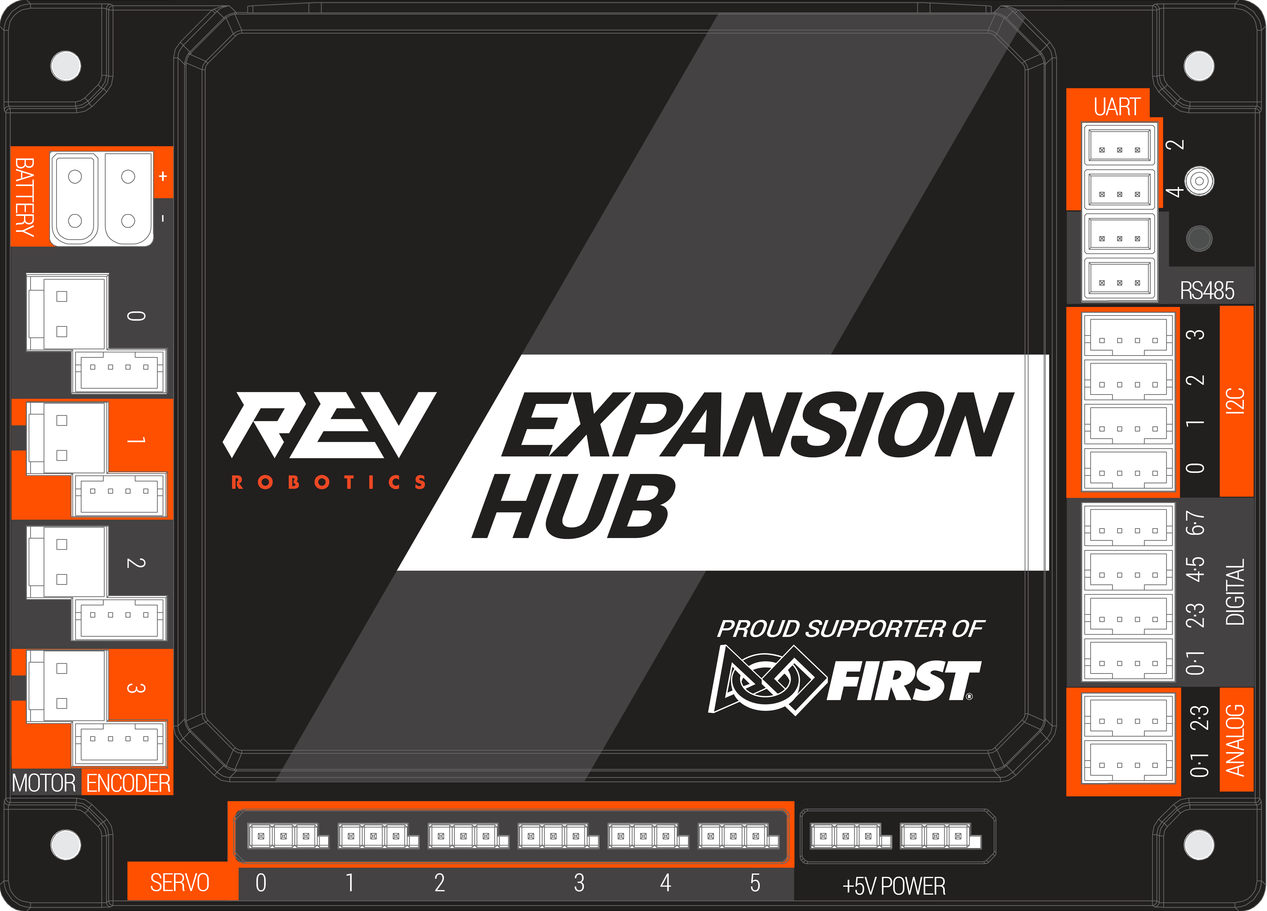
\includegraphics{1/images/expansion_hub_four.png}
    \caption{Image of the REV Expansion Hub. We will go over the specifics of what each port is for in this section.}
\end{figure}
The REV Expansion Hub is the core of the current control system. This is the piece of hardware which controls the various pieces of hardware on the bot. 
\subsection{Phones}
\subsection{Gamepad}
\subsection{Motors}
\subsection{Servos}
\subsection{Sensors}
\subsection{Wheels}
\subsection{Wiring}
\end{document}
